\documentclass{beamer}
\usetheme{Copenhagen}
\usepackage{tikz}
\usepackage{multirow}
\usepackage{graphicx}
\usepackage{epstopdf}
\graphicspath{{img/}}

\title[Graph Structure in the Web --- Revisited]{Graph Structure in the Web --- Revisited}
\subtitle{or A Trick of the Heavy Tail}
\institute{}
\author[by Chen Shaoyuan]{Author: Robert Meusel, Sebastiano Vigna, Oliver Lehmberg, Christian Bizer}
\date{September 30, 2017}

\begin{document}
  \begin{frame}
    \titlepage
  \end{frame}

  \section{Overall}
  \begin{frame}{Overall}
    \begin{itemize}
      \item Crawled in 2012
      \item Containing 3.5 billion web pages and 128.7 billion links
      \item Analyzed features of the Web graph, including
      \begin{itemize}
        \item degrees (indegree, outdegree)
        \item components (weekly connected, strongly connected)
        \item diameter and distances
      \end{itemize}
    \end{itemize}
  \end{frame}

  \begin{frame}{Overall}{Intuition}
    It is natural to treat the web as graph.
    \begin{itemize}
      \item Nodes correspond to static pages on the Web
      \item Arcs correspond to links between pages
    \end{itemize}
    \pause
    By studying Web graph, we can
    \begin{itemize}
      \item design crawl strategies on the web
      \item improve PageRank algorithms
      \item understand the sociology of content creation on the web
      \item predict the evolution of the web
    \end{itemize}
  \end{frame}

  \section{Bow-Tie Structure}
    \begin{frame}{Bow-Tie Structure}{Components of the web graph}
    Several studies confirm the existence of a large strongly connected components, significantly larger than any other components. \par
    \pause
    \begin{center}
    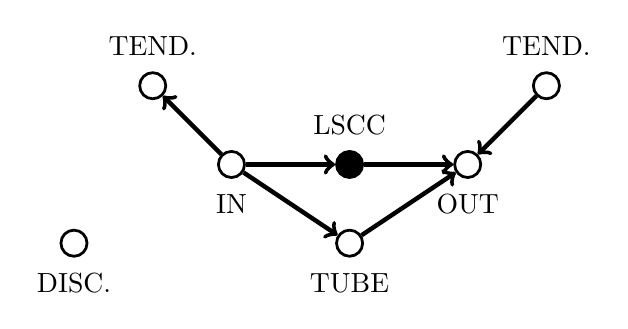
\begin{tikzpicture}[line width = 1pt,
                        solid/.style = {circle, draw, fill = black, minimum size = 0.1cm},
                        empty/.style = {circle, draw, fill = white, minimum size = 0.1cm}]p
      \node [empty] (a1) at (0, 1){};       \node at (0, 1.5) {TEND.};p
      \node [empty] (a2) at (1, 0){};       \node at (1, -0.5) {IN};
      \node [solid] (a3) at (2.5, 0){};     \node at (2.5, 0.5) {LSCC};
      \node [empty] (a4) at (4, 0){};       \node at (4, -0.5) {OUT};
      \node [empty] (a5) at (5, 1){};       \node at (5, 1.5) {TEND.};
      \node [empty] (a6) at (2.5, -1){};    \node at (2.5, -1.5) {TUBE};
      \node [empty] (a7) at (-1, -1){};     \node at (-1, -1.5) {DISC.};
      \draw [->, ultra thick] (a2) -- (a1);
      \draw [->, ultra thick] (a2) -- (a3);
      \draw [->, ultra thick] (a3) -- (a4);
      \draw [->, ultra thick] (a5) -- (a4);
      \draw [->, ultra thick] (a2) -- (a6);
      \draw [->, ultra thick] (a6) -- (a4);
    \end{tikzpicture}
    \end{center}
  \end{frame}

  \begin{frame}{Bow-Tie Structure}{Components of Bow-Tie Structure}
    \begin{itemize}
      \item LSCC: large strongly connected components
      \item IN: nodes that can reach LSCC
      \item OUT: nodes that can be reached from LSCC
      \item TENDRILS: nodes that can either be reached from IN, or can reach OUT
      \item TUBES: nodes that lie on paths from IN to OUT, without passing LSCC
      \item DISCONNECTED: nodes that are not weakly connected to LSCC
    \end{itemize}
  \end{frame}

  \begin{frame}{Bow-Tie Structure}{A Typical Bow-Tie Structure}
    \begin{center}
    \includegraphics[width = 8.5cm]{bow-tie-structure.pdf}
    \end{center}
  \end{frame}

  \begin{frame}{Bow-Tie Structure}{Comparison of Sizes of Bow-Tie Components}
    \begin{center}
    \begin{table}
    \begin{tabular}{|c|c|c|c|c|}
      \hline
        &  \multicolumn{2}{c|}{Common Crawl 2012}  &  \multicolumn{2}{c|}{Broder \emph{et al.} (2000)}  \\ \hline
      Component & \# nodes (k) & \% nodes &  \# nodes (k) & \% nodes \\ \hline
      LSCC & 1 827 543 & 51.28 & 56 464 & 27.74    \\
      IN & 1 138 869 & 31.96 & 43 343 & 21.29   \\
      OUT & 215 409 & 6.05 & 43 166 & 21.21  \\
      TENDRILS & 164 465 & 4.61 & 43 798 & 21.52  \\
      TUBES & 9 099 & 0.26 & - & - \\
      DISC. & 208 217 & 5.84 & 16 778 & 8.24 \\ \hline
    \end{tabular}
    \caption{Comparison of sizes of bow-tie components}
    \end{table}
    \end{center}
  \end{frame}

  \begin{frame}{Bow-Tie Structure}{Phenomena \& Analysis}
    \begin{enumerate}[1]
      \item The size of LSCC has almost doubled.
      \pause
      \begin{itemize}
        \item The web has become more dense and connected.
      \end{itemize}
      \pause
      \item The IN component has become much larger than OUT component in size.
      \pause
      \begin{itemize}
        \item Crawl methodology (esp. crawl seeds)
        \item Small websites?
      \end{itemize}
    \end{enumerate}
  \end{frame}

  \begin{frame}{Bow-Tie Structure}{Comparison between Page Graph and PLD Graph}
    \begin{center}
    \begin{table}
    \begin{tabular}{|c|c|c|c|c|}
      \hline
        &  \multicolumn{2}{c|}{page graph}  &  \multicolumn{2}{c|}{PLD graph}  \\ \hline
      Component & \# nodes (M) & \% nodes &  \# nodes (M) & \% nodes \\ \hline
      LSCC & 1 828 & 51.28 & 22.3 & 51.94    \\
      IN & 1 139 & 31.96 & 3.3 & 7.65   \\
      OUT & 215 & 6.05 & 13.3 & 30.98  \\
      TENDRILS & 164 & 4.61 & 0.5 & 1.20  \\
      TUBES & 9 & 0.26 & 0.2 & 0.04 \\
      DISC. & 208 & 5.84 & 3.5 & 8.20 \\ \hline
    \end{tabular}
    \caption{Comparison between Page Graph and PLD Graph}
    \end{table}
    \end{center}
  \end{frame}

  \section{Degree Distribution}
  \begin{frame}{Degree Distribution}{the Power Law}
    Broder \emph{et al.} claimed that the degree distribution follows the power law, both indegree and outdegree. \par
    \pause
    \begin{block}{Power Law}
    $$ f(x) = ax^{-k}, k > 1$$
    \end{block}
    \pause
    \begin{itemize}[<+->]
      \item Scale invariance: $ f(cx) = a(cx)^{-k} = c^{-k} f(x) \propto f(x)$
      \item Heavy-tailed, 80--20 rule
      \item Well-defined mean exists only when $k > 2$
      \item Linear in log-log plot
    \end{itemize}
  \end{frame}

  \begin{frame}{Degree Distribution}{Why not Power Law?}
    \begin{figure}
        \includegraphics[width = 7cm]{dist_plot.pdf}
        \caption{Log-log plot of degree distributions}
    \end{figure}
  \end{frame}
  
  \begin{frame}{Degree Distribution}{Why not Power Law?}
    Problems:
    \pause
    \begin{itemize}
      \item The conclusion was drawn just by the approximate linear shape in log-log plot.
      \pause
      \item The concavity in the left part cannot be explained.
      \begin{itemize}
        \item There are not so much pages with few hyperlinks as expected.
      \end{itemize}  
      \pause
      \item The data points in the right part deviate the line.
      \begin{itemize}
        \item The number of pages with huge number of hyperlinks decreases rapidly as the number of links increases. (hyperpolynomial decrease)
      \end{itemize}
    \end{itemize}
  \end{frame}
  
  \begin{frame}{Degree Distribution}{Other Conclusions}
    In fact, indegree distribution fits the power law better than outdegree. 
    \pause
    \begin{itemize}[<+->]
      \item The concavity is more obvious in indegree distribution.
      \item The indegree distribution curve drops much faster than outdegree , when degree grows large.
    \end{itemize}
    \pause
    Why?
    \pause
    \begin{itemize} [<+->]
      \item technical limitations
      \item although the average degree has significantly increased by 5
    \end{itemize}
  \end{frame}
  
  \section{Diameter and Distances}
  \begin{frame}{Diameter and Distances}
    \begin{itemize}[<+->]
      \item The average distance is 12.84.
      \item The harmonic diameter is 24.43.
      \item The average distance was 16.12 in 2000, reported by Broter \emph{et al.}
      \item ``Small-world network''
    \end{itemize}
  \end{frame}
  
  \section{References}
  \begin{frame}{References}
    \scriptsize
    \begin{enumerate}[\lbrack 1\rbrack]
      \item R. Meusel, S. Vigna, O. Lehmberg, and C. Bizer. Graph structure in the Web --- Revisited: A trick of the heavy tail. \emph{Proceedings of WWW Companion '14}, 427--432, 2014.
      \item A. Broder, R. Kumar, F. Maghoul, P. Raghavan, S. Rajagopalan, R. Stata, A. Tomkins and J. Wiener. Graph structure in the Web: experiments and models. \emph{Computer Networks}, 33(1--6):309-320, 2000.
      \item O. Lehmberg, R. Meusel and C. Bizer. Graph Structure in the Web --- Aggregated by Pay-Level Domain. \emph{Proceedings of the 1024 ACM conference on Web Science}, 119--128, 2014.
      \item D. Donato, S. Leonardi, S. Millozzi, and P. Tsaparas. Mining the inner structure of the web graph. \emph{WebDB}, 145-150, 2005.
    \end{enumerate}
  \end{frame}
\end{document}
